\documentclass{article}
\usepackage{nips10submit_e,times}
\usepackage{algorithm,algorithmic}

\title{Supplementary material: Online variational inference for state-space models
with point process observations}


\usepackage[dvips]{epsfig}
\usepackage{url}
\usepackage{amsmath}
\usepackage{amsfonts}
\usepackage{amssymb}
%\usepackage{graphicx}
\usepackage{bm}
\usepackage{array}
\usepackage{subfigure}
\usepackage{float}
\floatstyle{ruled}
\newfloat{algorithm}{htbp}{loa}[section]
\floatname{algorithm}{Algorithm}

\newcolumntype{x}[1]{%
>{\centering\hspace{0pt}}p{#1}}%

\newcounter{remarkcounter}
%\addtocounter{remarkcounter}{1}

\newtheorem{theorem}{Theorem}
\newtheorem{lemma}[theorem]{Lemma}
\newtheorem{proposition}[theorem]{Proposition}
\newtheorem{corollary}[theorem]{Corollary}
\newtheorem{remark}[remarkcounter]{Remark}


\newenvironment{proof}[1][Proof]{\textbf{#1.} }{\ \rule{0.5em}{0.5em}}
\newenvironment{definition}[1][Definition]{\begin{trivlist}
\item[\hskip \labelsep {\bfseries #1}]}{\end{trivlist}}
\newenvironment{example}[1][Example]{\begin{trivlist}
\item[\hskip \labelsep {\bfseries #1}]}{\end{trivlist}}
%\newenvironment{remark}[1][Remark]{\begin{trivlist}
%\item[\hskip \labelsep {\bfseries #1}]}{\end{trivlist}}

\newcommand{\Azero} {\textsl{} A}
\newcommand{\Bzero} {\textsl{} B_0}
\newcommand{\Tkk} {{\bf T}_{k-1}}
\newcommand{\Jk} {{\bf J}_{k}}
\newcommand{\Ak} {{\bf A}_k}
\newcommand{\Akplusone} {{\bf A}_{k+1}}
\newcommand{\Akk} {{\bf A}_{k-1}}
\newcommand{\Amat} {{\bf A}}
\newcommand{\Cmat} {{\bf C}}
\newcommand{\thetab} {{\bm \theta}}
\newcommand{\chib} {{\bm \chi}}
\newcommand{\rhob} {{\bm \rho}}
\newcommand{\thetabj} {{\bm \theta}_j}
\newcommand{\thetabjj} {{\bm \theta}_{j-1}}
\newcommand{\thetabk} {{\bm \theta}_k}
\newcommand{\thetabkk} {{\bm \theta}_{k-1}}
\newcommand{\thetabkkk} {{\bm \theta}_{k-2}}
\newcommand{\thetabkkkk} {{\bm \theta}_{k-3}}
\newcommand{\thetabkkhat} {{\hat{\bm \theta}}_{k-1}}
\newcommand{\thetabkkkhat} {{\hat{\bm \theta}}_{k-2}}
\newcommand{\thetabkkkkhat} {{\hat{\bm \theta}}_{k-3}}
\newcommand{\Thetak} {\Theta_{k}}
\newcommand{\Thetakk} {\Theta_{k-1}}
\newcommand{\Thetakkk} {\Theta_{k-2}}
\newcommand{\phib} {{\bm \phi}}
\newcommand{\psib} {{\bm \psi}}
\newcommand{\zetab} {{\bm \zeta}}
\newcommand{\zetabk} {{\bm \zeta}_k}
\newcommand{\Phib} {{\bm \Phi}}
\newcommand{\z} {{\bf z}}
\newcommand{\un} {{\bf u_n}}
\newcommand{\s} {{\bf s}}
\newcommand{\rr} {{\bf r}}
\newcommand{\ab} {{\bf a}}
\newcommand{\aj} {{\bf a}_j}
\newcommand{\ai} {{\bf a}_i}
\newcommand{\aik} {{\bf a}_{i,k}}
\newcommand{\ajk} {{\bf a}_{j,k}}
\newcommand{\ajzero} {{\bf a}_{j,0}}
\newcommand{\aikk} {{\bf a}_{i,{k-1}}}
\newcommand{\ajkk} {{\bf a}_{j,{k-1}}}
\newcommand{\ajkkk} {{\bf a}_{j,{k-2}}}
\newcommand{\ajkplusone} {{\bf a}_{j,k+1}}
\newcommand{\ajkgivenk} {{\bf a}_{j,k|k}}
\newcommand{\ajkkgivenkk} {{\bf a}_{j,k-1|k-1}}
\newcommand{\sjk} {{\bf s}_{j,k}}
\newcommand{\x} {{\bf x}}
\newcommand{\e} {{\bf e}}
\newcommand{\w} {{\bf w}}
\newcommand{\W} {{\bf W}}
\newcommand{\y} {{\bf y}}
\newcommand{\q} {{\bf q}}
\newcommand{\Ik} {{\bf I}_k}
\newcommand{\ub} {{\bf u}}
\newcommand{\Qm} {{\mathcal{Q}}}
\newcommand{\mub} {{\bm \mu}}
\newcommand{\mubk} {{\bm \mu_k}}
\newcommand{\mubkk} {{\bm \mu_{k-1}}}	
\newcommand{\mubkoff} {{\bm \mu_k'}}
\newcommand{\mubkkoff} {{\bm \mu_{k-1}'}}
\newcommand{\mubAkk} {{\bm \mu^A_{k-1}}}
\newcommand{\mubAkkk} {{\bm \mu^A_{k-2}}}
\newcommand{\mubAjk} {{\bm \mu^A_{j,k}}}
\newcommand{\mubAjkk} {{\bm \mu^A_{j,k-1}}}
\newcommand{\mubAjkkk} {{\bm \mu^A_{j,k-2}}}
\newcommand{\mubktilde} {\widetilde{\bm \mu_k}}
\newcommand{\mubthetakk} {{\bm \mu^{\thetab}_{k-1}}}
\newcommand{\mubthetakkk} {{\bm \mu^{\thetab}_{k-2}}}
\newcommand{\vv} {{\bm \nu}}
\newcommand{\vvm} {{\mathcal {\bm \upsilon}}}
\newcommand{\kappab} {{\mathcal {\bm \kappa}}}
\newcommand{\alphainv} {\alpha^{-1}}
\newcommand{\Jcost} {{\mathcal J}}
\newcommand{\xdot} {{\bf \dot{x}}}
\newcommand{\Vm} {{\bf \mathcal{V}}}
\newcommand{\expect} {\mathbb{E}}
\renewcommand{\Re} {\mathbb{R}}
\newcommand{\Var} {\mathrm{Var}}
\newcommand{\N} {\mathcal{N}}
\newcommand{\Zplus} {\mathbb{Z}^+}
\newcommand{\ltheta} {{l_\thetab}}
%\renewcommand{\int} {\int}

\newcommand{\Psixinv} {{\bf \Psi_x^{-1}}}
\newcommand{\Psix} {{\bf \Psi_x}}
\newcommand{\Psie} {{\bf \Psi_e}}
\newcommand{\Psitheta} {{\bf \Psi_\theta}}
\newcommand{\Sigmawinv} {{\bf \Sigma_w^{-1}}}
\newcommand{\Sigmaw} {{\bf \Sigma_w}}
\newcommand{\SigmaA} {{\bf \Sigma_A}}
\newcommand{\Sigmamu} {{\bf \Sigma_{\mu}}}
\newcommand{\Sigmarho} {{\bf \Sigma_{\rho}}}
\newcommand{\Sigmaalpha} {{\bf \Sigma_{\alpha}}}
\newcommand{\Sigmarhohat} {{\bf \hat{\Sigma_{\rho}}}}
\newcommand{\Sigmab} {{\bf \Sigma}}
\newcommand{\Sigmabk} {{\bf \Sigma_k}}
\newcommand{\Sigmabktilde} {\widetilde{\bf \Sigma_k}}
\newcommand{\Sigmakk} { \Sigma_{k-1}}
\newcommand{\Sigmakkinv} { \Sigma_{k-1}^{-1}}
\newcommand{\Sigmabkk} {{\bf \Sigma_{k-1}}}
\newcommand{\Sigmabkkstar} {{\bf \Sigma_{k-1}^*}}
\newcommand{\Sigmabkinv} {{\bf \Sigma_k^{-1}}}
\newcommand{\Sigmabkkinv} {{\bf \Sigma_{k-1}^{-1}}}
\newcommand{\Sigmabkoff} {{\bf \Sigma_k'}}
\newcommand{\Sigmabkoffinv} {{\bf \Sigma_{k}'^{-1}}}
\newcommand{\Sigmabkkoff} {{\bf \Sigma_{k-1}'}}
\newcommand{\Sigmabkkoffinv} {{\bf \Sigma_{k-1}'^{-1}}}
\newcommand{\Sigmabthetakk} {{\bf \Sigma^{\thetab}_{k-1}}}
\newcommand{\Sigmabek} {{\bf \Sigma^{e}_{k}}}
\newcommand{\Sigmabekk} {{\bf \Sigma^{e}_{k-1}}}
\newcommand{\Sigmabekkk} {{\bf \Sigma^{e}_{k-2}}}
\newcommand{\Sigmabthetakkinv} {{\bf \Sigma^{\thetab^{-1}}_{k-1}}}
\newcommand{\Sigmabthetakkkinv} {{\bf \Sigma^{\thetab^{-1}}_{k-2}}}
\newcommand{\Sigmabthetakkk} {{\bf \Sigma^{\thetab}_{k-2}}}
\newcommand{\Sigmav} {{\bf \Sigma_v}}
\newcommand{\betab} {{\bm \beta}}
\newcommand{\gammab} {{\bm \gamma}}

\newcommand{\A}{{\bf A}}
\newcommand{\Astar}{{\bf A^*}}
\newcommand{\Atilde}{{\bf \tilde{A}}}
\newcommand{\Ahat}{{\bf \hat{A}}}
\newcommand{\ba}{{\bf a}}
\newcommand{\B}{{\bf B}}
\newcommand{\E}{{\bf E}}
\newcommand{\D}{{\bf D}}
\newcommand{\F}{{\bf F}}
\newcommand{\FF}{{\mathcal F}}
\newcommand{\OO}{{\mathcal O}}

\newcommand{\bb}{{\bf b}}
\newcommand{\f}{{\bf f}}
\newcommand{\ft}{\tilde{f}}
\newcommand{\pt}{\tilde{p}}
\newcommand{\phat}{\hat{p}}
\newcommand{\h}{{\bf h}}
\newcommand{\bu}{{\bf u}}
\newcommand{\ud}{{\bf u_d}}
\newcommand{\bv}{{\bf v}}
\newcommand{\zk}{{\bf z_k}}
\newcommand{\zkk}{{\bf z_{k-1}}}
\newcommand{\C}{{\bf C}}
\newcommand{\CA}{{\bf C^A}}
\newcommand{\Ck}{{\bf C}_k}
\newcommand{\Ckk}{{\bf C}_{k+1}}
\newcommand{\I}{{\bf I}}
\newcommand{\G}{{\bf G}}
\newcommand{\Sk}{{\bf S}_k}
\newcommand{\Wk}{{\bf W}_k}
\newcommand{\Wkk}{{\bf W}_{k-1}}
\newcommand{\Z}{{\bf Z}}
\newcommand{\Hk}{{\bf H_k}}
\newcommand{\Q}{{\bf Q}}
\newcommand{\Qinv}{{\bf Q}^{-1}}
\newcommand{\Qdinv}{{\bf Q}^{-2}}
\newcommand{\R}{{\bf R}}
\newcommand{\Rinv}{{\bf R}^{-1}}
\newcommand{\Kk}{{\bf K_k}}
\newcommand{\Kkplusone}{{\bf K_{k+1}}}
\newcommand{\Y}{\mathcal{Y}}
\newcommand{\Yj}{\mathcal{Y}_j}
\newcommand{\Yk}{\mathcal{Y}_k}
\newcommand{\Ykk}{\mathcal{Y}_{k-1}}
\newcommand{\Ykkk}{\mathcal{Y}_{k-2}}
\newcommand{\X}{\mathcal{X}}
\newcommand{\Xk}{\mathcal{X}_k}
\newcommand{\Xkk}{\mathcal{X}_{k-1}}
\newcommand{\Xkkk}{\mathcal{X}_{k-2}}
\newcommand{\Xkkkk}{\mathcal{X}_{k-3}}
\newcommand{\Asetk}{\mathcal{A}_k}
\newcommand{\Asetkk}{\mathcal{A}_{k-1}}
\newcommand{\zero}{{\bf 0}}
\newcommand{\Thetahatkk}{{\hat{\Theta}_{k-1}}}
\newcommand{\Thetahatkkk}{{\hat{\Theta}_{k-2}}}
\newcommand{\Thetahatkkkk}{{\hat{\Theta}_{k-3}}}


\newcommand{\xstar}{{\bf x^*}}
\newcommand{\Dx}{{\bf \Delta x}}
\newcommand{\Dxdot}{{\bf \Delta \dot{x}}}
\newcommand{\xj}{{\bf x}_j}
\newcommand{\xjj}{{\bf x}_{j-1}}
\newcommand{\xk}{{\bf x}_k}
\newcommand{\xkk}{{\bf x}_{k-1}}
\newcommand{\xkkk}{{\bf x}_{k-2}}
\newcommand{\xkkkk}{{\bf x}_{k-3}}
\newcommand{\ek}{{\bf e}_k}
\newcommand{\ekk}{{\bf e}_{k-1}}
\newcommand{\yk}{{\bf y}_k}
\newcommand{\ykk}{{\bf y}_{k-1}}
\newcommand{\uk}{{\bf u}_k}
\newcommand{\wk}{{\bf w}_k}
\newcommand{\vk}{{\bf v}_k}
\newcommand{\Pk}{{\bf P}_k}
\newcommand{\Pkplusone}{{\bf P}_{k+1}}
\newcommand{\xkplusone}{{\bf x}_{k+1}}
\newcommand{\xkprev}{{\bf x}_{k-1}}

\newcommand{\wkprev}{{\bf w}_{k-1}}
\newcommand{\vkprev}{{\bf v}_{k-1}}
\newcommand{\xhat}{{\bf \hat{x}}}
\newcommand{\xkhat}{{\bf \hat{x}}_k}
\newcommand{\xkhatprev}{{\bf \hat{x}}_{k-1}}
\newcommand{\xktilde}{{\bf \widetilde{x}}_k}
\newcommand{\ekprior}{{\bf e_{k}^-}}
\newcommand{\ekpriorplusone}{{\bf e}_{k+1}^{-}}
\newcommand{\Pkprior}{{\bf P_{k}^-}}
\newcommand{\Pkpriorplusone}{{\bf P}_{k+1}^-}
\newcommand{\xkhatprior}{{\bf \hat{x}}_k^-}
\newcommand{\xkhatpriorplusone}{{\bf \hat{x}}_{k+1}^-}
\newcommand{\xzerohatprior}{{\bf \hat{x}}_0^-}
\newcommand{\Pzeroprior}{{\bf P}_{0}^-}

\newcommand{\xhatatkgivenk}{{\bf \hat{x}}_{k \mid k}}
\newcommand{\xhatatkkgivenk}{{\bf \hat{x}}_{k-1 \mid k}}
\newcommand{\xhatatkkgivenkk}{{\bf \hat{x}}_{k-1 \mid k-1}}
\newcommand{\xhatatkgivenN}{{\bf \hat{x}}_{k \mid N}}
\newcommand{\xhatatNgivenN}{{\bf \hat{x}}_{N \mid N}}
\newcommand{\xhatatkplusNgivenk}{{\bf \hat{x}}_{k + N \mid k}}
\newcommand{\xhatatkplusonegivenN}{{\bf \hat{x}}_{k + 1 \mid N}}
\newcommand{\xhatatkplusonegivenk}{{\bf \hat{x}}_{k + 1 \mid k}}
\newcommand{\Patkgivenk}{{\bf {P}}_{k \mid k}}
\newcommand{\PatkgivenN}{{\bf {P}}_{k \mid N}}
\newcommand{\PatNgivenN}{{\bf {P}}_{N \mid N}}
\newcommand{\PatkplusNgivenk}{{\bf {P}}_{k + N \mid k}}
\newcommand{\Patkplusonegivenk}{{\bf {P}}_{k + 1 \mid k}}
\newcommand{\PatkplusonegivenN}{{\bf {P}}_{k + 1 \mid N}}

\newcommand{\ent}{\mathcal{H}}
\newcommand{\info}{\mathcal{I}}

\newcommand{\obsmodel}{f(\yk | \thetabk,\Ykk)}
\newcommand{\evolmodel}{f(\thetabk | \thetabkk)}
\newcommand{\filterdist}{f(\thetabk | \Yk)}
\newcommand{\predictdist}{f(\thetabk | \Ykk)}
\newcommand{\smoothdist}{f(\thetabkk | \Yk)}


\usepackage{color}
\newcommand{\red}{\textcolor{red}}
\newcommand{\blue}{\textcolor{blue}}
\newcommand{\green}{\textcolor{green}}
\bibliographystyle{IEEEtran}	



\newcommand{\fix}{\marginpar{FIX}}
\newcommand{\new}{\marginpar{NEW}}


\begin{document}

\maketitle

\section{Introduction}

The supplementary material presented here outlines the derivations of most of the equations used in the submission.  Most of the work in this regard is carried on the lines of~\cite{Beal_2003b}. A brief outline of the 2-stage Gibbs sampler used is also given together with some further results.

\section{The forward pass} \label{sec:FP}

Initialise $x_{1|1}$ and set $\Sigma_{1|1} = \kappa$ where $\kappa$ is indicative of the uncertainty on the initial state. The forward pass is given by~\cite{Beal_2003b}

\begin{equation*}
p(x_k | \Yk) \propto \int {dx_{k-1}} p(x_{k-1} | \Ykk)\exp{\langle \ln p(x_k | x_{k-1},\thetab) p(\yk | x_k,\thetab)\rangle}
\end{equation*}

\noindent where $p(x_k | x_{k-1},\thetab) = \N_{x_k}(\rho x_{k-1} + \alpha I_k, \sigma^2_{\epsilon})$ and $p(x_{k-1} | \Ykk) = \N_{x_{k-1}}(x_{k-1|k-1} | \sigma^{2}_{k-1|k-1})$. We can use the property of logarithms and linearity in expectation to start off by considering the product $p(x_k | x_{k-1},\thetab)p(x_{k-1} | \Ykk)$ which is normal in $x_{k-1}$ with precision

\begin{equation*}
\overline{\sigma}^{-2}_{k-1} = \sigma^{-2}_{k-1} + \langle \rho^2 \rangle\sigma^{-2}_\epsilon
\end{equation*}

\noindent and mean

\begin{equation*}
\overline{x}_{k-1} = \overline{\sigma}^{2}_{k-1}(x_{k-1 | k-1}\sigma^{-2}_{k-1|k-1} + \langle \rho \rangle x_k  \sigma^{-2}_\epsilon - \langle \rho\alpha \rangle I_k  \sigma^{-2}_\epsilon)
\end{equation*}

We then marginalise out $x_{k-1}$ to get

\begin{equation}\label{eq:Forward1}
p(x_k | \Yk) \propto \N_{x_k}(\tilde{x_k}, \tilde{\sigma}^2_k) \exp(\langle \ln p(\yk | x_k,\thetab)\rangle )
\end{equation}

\noindent where

\begin{equation*}
\tilde{\sigma}^{-2}_k = \sigma^{-2}_{\epsilon} - \langle \rho \rangle^2 \overline{\sigma}^{2}\sigma^{-4}_{\epsilon}
\end{equation*}


and

\begin{equation*}
\tilde{x_k} = \tilde{\sigma}^{2}_k\bigg(\overline{\sigma}^{2}\langle \rho \rangle \sigma^{-2}_{\epsilon}[x_{k-1|k-1}\sigma^{-2}_{k-1|k-1} - \langle \rho \alpha \rangle I_k \sigma^{-2}_{\epsilon}] + \langle \alpha \rangle I_k \sigma^{-2}_{\epsilon}\bigg)
\end{equation*}

To get the forward pass estimates we need to evaluate (\ref{eq:Forward1}). Since the observation equation is nonlinear we choose to approximate the product of the distributions to a Gaussian so that

\begin{equation}\label{eq:Forward2}
\langle \ln p(\yk | x_k, \thetab)\rangle + \ln \N_{x_k}(\tilde{x_k} , \tilde{\sigma}^2_k) = \ln \N_{x_k}(x_{k|k} , \sigma^2_{k|k})
\end{equation}

\noindent where, we recall

\begin{equation*}
 p(\yk | x_k, \thetab) = \prod_{c=1}^C\Delta\exp(\mu + \beta^cx_k)^{y_k^c}\exp(-\exp(\mu + \beta^cx_k)\Delta)
\end{equation*}

We next find the first derivative of (\ref{eq:Forward2}) evaluated at $x_k = x_{k|k}$ to find an expression for $x_{k|k}$. We then find the second derivative evaluated at the same point to find an expression for $\sigma^2_{k|k}$. As shown in the main work, a nonlinear optimiser is needed to evaluate $x_{k|k}$.

\section{The backward pass}

Initialise with $\sigma^{*^2} = \kappa$ where $\kappa$ is large and $x^*_{K} = x_{K|K}$ if carried out after the forward pass (see below). The backward pass is given by the recursion \cite{Beal_2003b}

\begin{equation*}
p(\y_{k+1:K} | x_k) = \int dx_{k+1} p(\y_{k+2:K} | x_{k+1}) \exp{\langle \ln p(x_{k+1} | x_{k},\thetab) p(\y_{k+1} | x_{k+1},\thetab)\rangle}
\end{equation*}

\noindent where $p(x_{k+1} | x_{k},\thetab) = \N_{x_{k+1}}(\rho x_k + \alpha I_{k+1}, \sigma^2_{\epsilon})$ and $p(\y_{k+2:K} , x_{k+1}) = \N_{x_{k+1}}(x^*_{k+1} | \sigma^{*^{2}}_{k+1})$. We can use the property of logarithms and linearity in expectation to start off by considering the product $p(\y_{k+2:K} | x_{k+1})\exp(\ln \langle p(\y_{k+1} | x_{k+1},\thetab) \rangle)$ which we approximate to a normal distribution centred at $x'_{k+1}$ with variance $\sigma'^2_{k+1}$. We do this in exactly the same way as Section \ref{sec:FP} but, this time, leaving the point about which we are linearising $\hat{x}_{k+1}$ free to obtain the expressions

\begin{subequations}
\begin{equation}
\begin{array}{rcl}
x'_{k+1} &=& \displaystyle \hat{x}_{k+1} + \sigma'^2_{k+1}\bigg(\frac{x_{k+1}^* - \hat{x}_{k+1}}{\sigma^{2^*}_{k+1}} + \sum_{c=1}^C \bigg\{\langle\beta^c\rangle_{\pt(\beta^c)}y^c_{k+1} - \\[2ex]
 && ~~~~\displaystyle \Delta \langle \exp{\mu} \rangle_{\pt(\mu)} \frac{d}{dx_{k+1}}\left.\left[\langle \exp{x_{k+1}\beta^c} \rangle_{\pt(\beta^c)}\right]\right|_{x_{k+1} = \hat{x}_{k+1} }  \bigg\} \bigg) \label{eq:NL2}  \\
\end{array}
\end{equation}
\begin{equation}\label{eq:NL2b}
\sigma'^2_{k+1} = \left({\sigma}^{*^{-2}}_{k+1} + \sum_{c=1}^C \left\{\Delta  \langle \exp{\mu} \rangle_{\pt(\mu)} \frac{d^2}{dx_{k+1}^2}\left.\left[\langle \exp{x_{k+1}\beta^c} \rangle_{\pt(\beta^c)}\right]\right|_{x_{k+1} = \hat{x}_{k+1}}\right\}\right)^{-1}
\end{equation}
\end{subequations}

The choice of $\hat{x}_{k+1}$ bears a lot of weighting on the performance of the algorithm. One can set $\hat{x}_{k+1}$ = $x'_{k+1}$ resulting in a nonlinear optimisation problem. On the other hand one can linearise around the filtered estimate $x_{k+1|k+1}$ instead and this is what is quoted in the submitted work. The advantage is that no nonlinear optimisation is required to compute the backward message. However, now, the backward pass can no longer be carried out in parallel with the forward pass.

The next step is to find the product of this approximate distribution with $\exp (\langle \ln p(x_{k+1} | x_{k},\thetab)\rangle )$ which is easily shown to be proportional to

\begin{equation*}
\exp\bigg(-x_{k+1}^2(\sigma^{-2}_\epsilon + \sigma'^{-2}_{k+1})/2 + x_{k+1}\bigg[\langle \rho \rangle x_k\sigma^{-2}_\epsilon + \langle \alpha \rangle I_{k+1}\sigma^{-2}_\epsilon + x'_{k+1}\sigma'^{-2}_{k+1} \bigg] - \langle \rho^2 \rangle x_k^2\sigma^{-2}_\epsilon/2 - \langle \rho \alpha \rangle x_k I_{k+1}\sigma^{-2}_\epsilon  \bigg)
\end{equation*}

We then marginalise out $x_{k+1}$ to obtain the required normal distribution in $x_k$ with mean $x^*_k$ and variance $\sigma^{*^2}_k$. The initial state estimate can be updated using the same equations in~\cite{Smith_2003}.

\section{Computing the sufficient statistics in the VB-E step}

The smoothed estimate is easily computed by considering the product distribution of the forward pass and the backward pass. In particular we find that

\begin{equation*}
p(x_k | \Y_K) \propto p(x_k | \Yk)p(\y_{k+1:K} | x_k)
\end{equation*}

Since this is a product of Gaussian distributions the state estimate conditioned on all the data can be found and can be readily computed in the backward pass if this is carried out sequential to the forward pass. The results are shown in the submitted work. Next we compute the pairwise marginals

\begin{equation*}
p(x_k,x_{k+1}| \Y_K)\propto p(x_k|\Y_K)p(\y_{k+2:K} |x_{k+1})\exp(\langle \ln p(x_{k+1}|x_k,\thetab_{k+1})p(\y_{k+1}|x_{k+1},\thetab_{k+1}) \rangle)
\end{equation*}

We expand the logarithm of this quantity and approximate it to a multivariate normal distribution as follows

\begin{equation*}
\begin{split}
& -x_k^2(\sigma^{-2}_{k|k} + \langle \rho^2 \rangle \sigma^{-2}_\epsilon)/2 - x_{k+1}^2(\sigma^{*^{-2}}_{k+1} + \sigma^{-2}_\epsilon)/2 \\
& + x_k(x_{k|k}\sigma^{-2}_{k|k} + \langle \rho \alpha \rangle I_{k+1}\sigma^{-2}_\epsilon) + x_{k+1}(x_{k+1}^*\sigma^{*^{-2}}_{k+1} + \langle \alpha \rangle I_{k+1}\sigma^{-2}_\epsilon) \\
&  + x_kx_{k+1}\langle \rho \rangle \sigma^{-2}_\epsilon + \sum_{c=1}^C\bigg[\langle y_{k+1}^c(\mu + \beta^cx_{k+1}) - \exp(\mu + \beta^cx_{k+1}) \rangle \bigg] + const. \\
=& -\frac{1}{2}[x_k~~x_{k+1}]\left[\begin{array}{cc} a & b \\ b & d\end{array} \right]\left[ \begin{array}{c} x_k\\ x_{k+1} \end{array}\right] + \cdots
\end{split}
\end{equation*}

where on the right hand side we have excluded terms which will disappear on taking two derivatives. To find $a$ we take two derivatives with respect to $x_k$ and to find $d$ we take two derivatives with respect to $x_{k+1}$ evaluated at $x_{k+1} = x_{k+1 | K}$. To find $b$ we first differentiate with respect to $x_k$ and then with respect to $x_{k+1}$. We find the cross-covariance by extracting the diagonal element from the inverted precision matrix. The second moment is then found by adding the product of the smoothed pair to the cross-covariance. The result is shown in the submitted work.

\section{VB-M step}

\subsection{Updating the statistics over $\mu$}

The variational posterior over $\mu$ is given by

\begin{equation*}
\ln \pt(\mu) = \ln p(\mu) + \langle \sum_{c = 1}^C \sum_{k=1}^K y^c_k[\mu + \beta^c x_k] - \exp(\mu)\exp(\beta^cx_k)\Delta \rangle
\end{equation*}

\noindent where p($\mu$) is the prior over $\mu$ with mean $\mu_p$ and variance $\sigma^2_p$. We restrict the variational posterior to be Gaussian with mean $\hat{\mu}$ and variance $\sigma^2_\mu$. Using the same trick of differentiating once and twice to obtain the mean and variance of the updated distribution we obtain the expressions given in the submitted work.
In these expressions it is required to evaluate the quantity $\langle \exp(x_i\beta^c)\rangle$. From moment generating functions we know that

\begin{equation*}
\int \exp(xt) \N_{x}(\mu , \sigma^2) dx = \exp(\mu t + \sigma^2t^2/2)
\end{equation*}

We are concerned with the quantity

\begin{equation*}
\begin{split}
\langle \exp(x_i\beta^c)\rangle &= \int dx_i \Bigg[\int d\beta^c \N_{\beta^c}(\hat{\beta}_c, \sigma^2_{\beta^c}) \Bigg] \N_{x_i}(\hat{x}_i,\sigma^2_{x_i}) \\
& = \int dx_i\exp(\hat{\beta}_cx_i + \sigma^2_{\beta^c}x_i^2) \N_{x_i}(\hat{x}_i,\sigma^2_{x_i}) \\
& = \frac{1}{\sqrt{2\pi\sigma^2_{x_i}}}\int dx_i \exp(\hat{\beta}_cx_i + \sigma^2_{\beta^c}x_i^2 - (x_i - \hat{x}_i)^2/2\sigma^2_{x_i})
\end{split}
\end{equation*}

To help the derivation one can set

\begin{equation*}
\begin{split}
\tilde{\Sigma} &= (\sigma^{-2}_{x_i} - \sigma^2_{\beta^c})^{-1} \\
\tilde{\mu} &= \tilde{\Sigma}(\hat{x}_i\sigma^{-2}_{x_i} + \hat{\beta}^c)
\end{split}
\end{equation*}

\noindent before marginalising out $x_k$. After some algebraic manipulation the final result (with expectations taken under the appropriate distributions) is obtained as

\begin{equation*}
\langle \exp(\beta^cx_i)\rangle_{\pt(\X_K)\pt(\beta^c)} =
\sqrt{\frac{1}{1 - \sigma^2_{\beta^c}\sigma^2_{i|K}}}\exp\left(\frac{x_{i|K}^2\sigma^2_{\beta^c} + \hat{\beta^c}^2\sigma^2_{i|K} + 2\hat{\beta^c}x_{i|K}}{2(1 - \sigma^2_{\beta^c}\sigma^2_{i|K})} \right)
\end{equation*}




\subsection{Updating the statistics over $\beta^c$}

The variational posterior over $\beta^c$ is given by

\begin{equation*}
\ln \pt(\beta^c) = \ln p(\beta^c) + \langle \sum_{k=1}^K y^c_k[\mu + \beta^c x_k] - \exp(\mu)\exp(\beta^cx_k)\Delta \rangle
\end{equation*}

\noindent where $p(\beta^c)$ denotes the prior over $\beta^c$. Effecting the required derivatives we once again restrict the variational posterior to be Gaussian with mean and variance as given in the submitted work. The expectations required in this case are those of log normal distributions which are easy to compute. In particular we have that

\begin{equation*}
\langle \exp(\beta^cx_k) \rangle_{\pt(\Xk)} = \exp(\beta^cx_{k|K} + \beta^{c^2}\sigma^2_{k|K}/2)
\end{equation*}

and

\begin{equation*}
\langle \exp(\mu) \rangle_{\pt(\mu)} = \exp(\hat{\mu} + \sigma^2_{\mu}/2)
\end{equation*}

\subsection{Updating the statistics over $\rho$ and $\alpha$}

In the interest of brevity we omit the implementation details and refer the interested reader to~\cite{Beal_2003b} and to the derivation for the online VB filter in the next.

\section{Derivation of the online VB algorithm for SSPP models}

We have the following general expressions for the online variational posteriors

\begin{subequations}\label{eq:VBmarginals}
\begin{align}
 \pt(\Xk)&\propto \exp(\langle[\ln p(\Xk,\Yk,\Thetak)]\rangle_{\pt(\Thetak)}) \label{eq:xkmarginal}\\[1ex]
 \pt(\theta^i_k)&\propto \exp\bigg[\langle[\ln p(\Xk,\Yk,\Thetak)]\rangle_{\pt(\Xk)\pt(\Thetak^{/\theta_k^i})}\bigg] \label{eq:thetakmarginal}
\end{align}
\end{subequations}
\normalsize

 \noindent where $\pt(\Thetak^{/\theta_k^i})$ is the joint $\pt(\Thetak)$ without the variable $\theta_k^i$. To compute the above online we propose the following recursion

 \begin{equation} \label{eq:Convenient}
\pt(x_k) \propto\displaystyle\int{ dx_{k-1}}\pt(x_{k-1})\exp(\langle\ln p(x_k| x_{k-1},\thetab_k) p(\yk | x_k,\thetab_k)\rangle_{\pt(\thetab_k)})
\end{equation}

\begin{equation} \label{eq:Convenienttheta}
\begin{array}{l}
\pt(\theta^i_k)\propto\exp(\langle \ln p(\yk|x_k,\thetab_k)p(x_k|x_{k-1},\thetab_k)\rangle_{\pt(\Xk)\pt(\thetab_k^{/i})})  \\ [2ex]
~~~~~~~~~~~~~~~~~~~~~~~~ \times~ \exp(\langle\ln p(\theta^i_k|\theta^i_{k-1})\rangle_{\pt(\theta^i_{k-1})}) ~~~ i = 1 \dots d
\end{array}
\end{equation}

To show that the above holds we start off by considering the variational approximation of the state marginal which is given by


\begin{equation} \label{eq:Statemarginalposterior}
\begin{split}
 \pt(x_k)  &\propto  \displaystyle \int d\Xkk \exp( \langle \ln p(\Xk,\Thetak,\Yk) \rangle) \\
 & = \exp( \langle \ln p(\yk|x_k,\thetab_k) \rangle ) \int d\Xkk \exp( \ln \langle p(x_k | x_{k-1}, \thetab_k) p(\Xkk, \Thetak,\Ykk) \rangle)
\end{split}
\end{equation}
\normalsize

\noindent where the above expectations are taken with respect to the unknown parameters. The second term of the integrand can be also expanded, and by treating the conditional parameter distributions as constants relative to the distribution of interest, it can be shown that

\begin{equation} \label{eq:Recursionvision}
\begin{split}
\pt(x_k) \propto & \displaystyle \exp( \langle \ln p(\yk|x_k, \thetabk) \rangle ) \int dx_{k-1}  \bigg( \exp(\langle \ln p(x_k | x_{k-1}, \thetabkk) \rangle) \\
& \times \bigg[  \exp( \langle \ln p(\ykk|x_{k-1}, \thetabkk) \rangle ) \int d\Xkkk \exp(\langle \ln  p(x_{k-1} | x_{k-2}, \thetabkk) \rangle) \\
& \times \exp(\langle \ln p(\Xkkk, \Thetakk,\Ykkk) \rangle)        \bigg]\bigg)
\end{split}
\end{equation}


Recall that since we have restricted the approximate parameter posteriors to be conditional on the data up to the instant in which they were estimated, the distributions of the parameters do not need to be recomputed using the latest data which is available. In particular for any function $\psi(\cdot)$

\begin{equation*}
\langle \psi(\thetabkk) \rangle_{\pt(\Thetak)}  =  \langle \psi(\thetabkk)\rangle_{\pt(\thetabkk | \Ykk)}
\end{equation*}

\noindent which was computed in the previous iteration. Hence, in comparison to (\ref{eq:Statemarginalposterior}), it is clear that the terms in the square brackets of (\ref{eq:Recursionvision}) constitute the exact variational posterior marginal of the state at the previous time instant to give (\ref{eq:Convenient}). Equation (\ref{eq:Convenienttheta}) follows by application of the chain rule on~(\ref{eq:thetakmarginal}) where the likelihood term $p(\yk|x_k,\thetab_k)$ and the joint $p(\Xkk,\Thetak^{/\theta^i_k},\Ykk)$ are constant relative to the distribution of interest.

From this point onwards one needs to recompute the VB-E step and VB-M step for each time instant. The E-step remains effectively the same as in the offline case with the the expectations taken with respect to the parameters at the \emph{present} time instant (recall some iterative VB is required at each time step). The E-step is carried out only on the pair $(x_k,x_{k-1})$. The sufficient statistics in the online M-step require the smoothing of $x_{k-1}$ at each time instant (see below).

The parameter updates are also very similar to the offline case. The only difference is that the prior is no longer fixed (although a fixed prior can be introduced), rather, according to the parameter evolution equation, it is a Gaussian distribution with the mean of the previous estimate and a precision weighted by a forgetting factor $\lambda$. In the simulations shown, no iterations were deemed necessary in each time instant with the results remaining essentially unchanged when several iterations were employed.

We next describe the online VB-M step, however we omit the online VB-E step since it is essentially the same as in the offline case. For convenience we use the following notation

\begin{equation*}
\begin{split}
U_k &= I_k^2 \\
G_k &= I_k \langle x_{k-1} \rangle \\
M_k &= I_k \langle x_{k} \rangle \\
W_k &= \langle x_{k-1}^2 \rangle \\
S_k &= \langle x_{k}x_{k-1} \rangle \\
\end{split}
\end{equation*}



\subsection{Online updating of $\pt(\alpha_k)$}

Following (\ref{eq:Convenienttheta}) we have that

\begin{equation} \label{eq:alphamarg}
\begin{split}
\ln \pt(\alpha_{k}) &\propto \langle \ln p(\alpha_k | \alpha_{k-1})\rangle + \langle p(x_k | x_{k-1}, \alpha_k, \rho_k) \rangle \\
&= - \frac{\langle \alpha_{k} - \alpha_{k-1} \rangle^2}{2\lambda^{\alpha^{-1}}\sigma^2_{\alpha_{k-1}}}  - \frac{\langle x_k - \rho_k x_{k-1} - \alpha_{k}I_k\rangle^2}{2\sigma^2_\epsilon}
\end{split}
\end{equation}

\noindent where we could ignore the observation density by treating it as a constant since it is independent of $\alpha_k$. Since we are assuming conditional dependence between $\rho_k$ and $\alpha_k$, as a result of factorising $\pt(\rho_k\alpha_k) = \pt(\rho_k | \alpha_k)\pt(\alpha_k)$ the expectation of $\rho$ needs to be taken with respect to the conditional distribution which is defined as

\begin{equation}
\ln \pt(\rho_k | \alpha_k) = \ln \langle p(\rho_k | \rho_{k-1}) \rangle + \ln \langle p(x_k | x_{k-1}, \rho_k, \alpha_k) \rangle
\end{equation}

\noindent and from this we obtain the expressions

\begin{equation}\label{eq:rhocond}
\begin{split}
\sigma^2_{\rho_k | \alpha_k} &= \left[\frac{1}{\lambda^{\rho^{-1}}\sigma^2_{\rho_{k-1}}} + \frac{W_k}{\sigma^2_\epsilon} \right]^{-1} \\
\langle \rho_k \rangle_{\pt(\rho_k | \alpha_k)} &= \sigma^2_{\rho_k | \alpha_k}\left[\frac{S_k}{\sigma^2_\epsilon} + \frac{\hat{\rho}_{k-1}}{\lambda^{\rho^{-1}}\sigma^2_{\rho_{k-1}}} - \frac{\alpha_kG_k}{\sigma^2_\epsilon} \right]
\end{split}
\end{equation}

On substituting (\ref{eq:rhocond}) in (\ref{eq:alphamarg}) we obtain the following update for $\alpha_k$

\begin{equation}\label{eq:alphaupdate}
\begin{split}
\sigma^2_{\alpha_k} &= \bigg(\frac{1}{\lambda^{\alpha^{-1}}\sigma^{2}_{\alpha_{k-1}}} + \frac{U_k}{\sigma^{2}_\epsilon} - \frac{\sigma^2_{\rho_{k}|\alpha_k}G_k^2}{\sigma^{4}_\epsilon} \bigg)^{-1} \\
\hat{\alpha}_k &= \sigma^2_{\alpha_k} \bigg(\frac{\hat{\alpha}_{k-1}}{\lambda^{\alpha^{-1}}\sigma^{2}_{\alpha_{k-1}}} + \frac{M_k}{\sigma^{2}_\epsilon} - \frac{G_k}{\sigma^{2}_\epsilon}\left[
\frac{S_k\sigma^2_{\rho_{k}|\alpha_k}}{\sigma^{2}_\epsilon}  + \frac{\sigma^2_{\rho_{k}|\alpha_k}\hat{\rho}_{k-1}}{\lambda^{\rho^{-1}}\sigma^{2}_{\rho_{k-1}}} \right]\bigg)
\end{split}
\end{equation}

\subsection{Online updating of $\pt(\rho_k)$}

The statistics over $\rho_k$ are obtained by marginalising $\alpha_k$ from the joint as follows

\begin{equation}
 \pt(\rho_{k}) = \int d\alpha_k \pt(\rho_{k}| \alpha_k)\pt(\alpha_k)
 \end{equation}

$\pt(\rho_{k}| \alpha_k)$ is computed from (\ref{eq:rhocond}) and $\pt(\alpha_k)$ is known from (\ref{eq:alphaupdate}). The marginalisation is straightforward to give the following expressions

\begin{equation}
\begin{split}
\sigma^2_{\rho_k} &= \sigma^2_{\rho_k | \alpha_k}  + \frac{\sigma^2_{\alpha_k}\sigma^4_{\rho_k|\alpha_k}G_k^2}{\sigma^4_\epsilon} \\
\hat{\rho_k} &= \sigma^2_{\rho_k | \alpha_k} \left[\frac{S_k}{\sigma^2_\epsilon}  + \frac{\hat{\rho}_{k-1}}{\lambda^{\rho^{-1}}\sigma^2_{\rho_{k-1}}} - \frac{G_k\hat{\alpha}_k}{\sigma^2_\epsilon} \right]
\end{split}
\end{equation}


\subsection{Online updating of $\pt(\mu_k)$}

Following (\ref{eq:Convenienttheta}) we have that

\begin{equation}
\begin{split}
\ln \pt(\mu_{k}) &\propto \langle \ln p(\mu_k | \mu_{k-1})\rangle + \langle p(y_k | x_{k}, \mu_k, \betab_k) \rangle \\
&= - \frac{\langle \mu_{k} - \mu_{k-1} \rangle^2}{2\lambda^{\mu^{-1}}\sigma^2_{\mu_{k-1}}}  + \langle\sum_{c=1}^C y_k^c[\mu_k + \beta^c_kx_k] - \exp(\mu_k)\exp(\beta^c_kx_k)\Delta \rangle
\end{split}
\end{equation}

\noindent where we could ignore the state evolution density by treating it as a constant since it is independent of $\mu_k$.  On expanding and approximating around $\hat{\mu}_{k}$ we obtain the following update equations

\begin{equation}
\begin{split}
\hat{\mu_k} &= \hat{\mu}_{k-1} + \lambda^{\mu^{-1}}\sigma^2_{\mu_{k-1}}\sum_{c=1}^C \left(y^c_k - \Delta \langle \exp(\beta^c_kx_k)\rangle\exp(\hat{\mu}_k) \right)  \\
\sigma^2_{\mu_k} &= \left(\lambda^{\mu}\sigma^{-2}_{\mu_{k-1}} + \Delta\exp(\hat{\mu_{k}}) \sum_{c=1}^C \langle \exp(\beta^c_kx_k)\rangle\right)^{-1}
\end{split}
\end{equation}

\subsection{Online updating of $\pt(\beta^c_k)$}

Following the same reasoning as that for updating $\pt(\mu_k)$ the resulting equations are given as

\begin{equation}
\begin{split}
\hat{\beta}^c_k &= \hat{\beta}^c_{k-1} + \lambda^{\beta^{-1}}\sigma^2_{\beta^c_{k-1}}\left(y^c_k\langle x_k \rangle - \Delta\langle \exp \mu_k \rangle \frac{d}{d\beta^c_k}\left. \left[\langle \exp{x_{k}\beta^c_k}\rangle\right] \right| _{\beta^c_k = \hat{\beta}^c_k}  \right) \\
 \sigma^2_{\beta^c_k} &= \left(\lambda^{\beta}\sigma^{-2}_{\beta^c_{k-1}} + \Delta\langle \exp \mu_k \rangle \left[\frac{d^2}{d\beta^{c_k^2}} \left. \langle \exp{x_k\beta^c_k}\rangle \right| _{\beta^c_k = \hat{\beta}^c_k}\right]\right)^{-1}
\end{split}
\end{equation} 	


\section{Gibbs Sampler}

The full Bayesian treatment for the SSPP model attempts to infer the joint distribution of the
underlying states and parameters given the observations: $p(\X_{K},\thetab|\Y_{K})$. As a MCMC
approximation, the Gibbs sampler
is a standard formulation to approach such a distribution \cite{Carter_1994,Geweke_2001}, which
iteratively draws samples
from two conditional probability distributions: $p(\X_{K}|\Y_{K},\thetab)$ and $p(\thetab|\Y_{K},\X_{K})$.

For sampling the states, the distribution $p(\X_{K}|\Y_{K},\thetab)$ can be utilized
by sequentially drawing samples from $p(x_{k}|\X_{k^{-}},\Y_{K},\thetab)$, where $k=1,\cdots,K$ and
$\X_{k{-}}$ denotes the all states excluding  $x_{k}$. The details of the distribution are as follows.

\begin{align}
	&p(x_{k}|\X_{k^{-}},\Y_{K},\thetab) \\ \nonumber
	&\propto \left\{
	\begin{array}{ll}
		p(x_{k}|x_{k-1},\alpha,\rho,\sigma^{2}_{\varepsilon})
		p(x_{k+1}|x_{k},\alpha,\rho,\sigma^{2}_{\varepsilon}) 	
		\prod^{C}_{c=1}p(y^{c}_{k}|x_{k},\mu,\beta^c) & \textrm{if
		$k=1,\ldots,K-1$} \nonumber \\
		p(x_{k}|x_{k-1},\alpha,\rho,\sigma^{2}_{\varepsilon})
		\prod^{C}_{c=1}p(y^{c}_{k}|x_{k},\mu,\beta^c) & \textrm{if $k=K$}
	\end{array}\right.
\end{align}

Similar to the state estimation, the parameters posterior distribution $p(\thetab|\Y_{K},\X_{K})$
is approached by single-site updates, where parameters are updated one at a time.
Such conditionals are given as:

\begin{align}
	p(\rho|\Y_{k},\X_{K},\alpha,\sigma^{2}_{\varepsilon},\mu,\betab) &\propto
	p(x_{0})\prod^{K}_{k=1}p(x_{k}|x_{k-1},\rho,\alpha,\sigma^{2}_{\varepsilon})p(\rho) \\
	p(\alpha|\Y_{k},\X_{K},\rho,\sigma^{2}_{\varepsilon},\mu,\betab) &\propto
	p(x_{0})\prod^{K}_{k=1}p(x_{k}|x_{k-1},\rho,\alpha,\sigma^{2}_{\varepsilon})p(\alpha)\\
	p(\mu|\Y_{k},\X_{K},\rho,\alpha,\sigma^{2}_{\varepsilon},\betab) &\propto
	\prod^{C}_{c=1}\prod^{K}_{k=1}p(y^{c}_{k}|x_{k},\mu,\beta^{c})p(\mu) \\
	p(\beta_{c}|\Y_{k},\X_{K},\rho,\alpha,\sigma^{2}_{\varepsilon},\mu) &\propto
	\prod^{K}_{k=1}p(y^{c}_{k}|x_{k},\mu,\beta^{c})p(\beta^{c})
\end{align}

In this work, the prior for each parameter is set to be the uniform distribution.
The Gibbs sampler for the above conditional distributions is shown in Algorithm \ref{alg:Gibbs}

\begin{algorithm}
	\caption{\nonumber A Gibbs Sampler for the SSPP Model}
	\label{alg:Gibbs}
	\begin{algorithmic}
		\STATE \textbf{1}. Initialise $\X^{(0)}_{K}, \thetab^{(0)}$
		\STATE \textbf{2}. Sampling and updating
		\FOR{$n=0,\ldots,N-1$}
		\FOR{$k=1,\ldots,K$}
		\STATE Sample $x^{(n+1)}_{k}$ from
		$p(x_{k}|\X^{(n)}_{k^-},\Y_{K},\thetab^{(n)})$
		\ENDFOR
		\STATE \ Sample $\thetab^{(n+1)}$ from $p(\thetab|\Y_{K},\X^{(n+1)}_{K})$.
		\ENDFOR
	\end{algorithmic}
\end{algorithm}

Clearly, for the SSPP model it is unfeasible to directly draw samples from the above distributions.
We use the Metropolis-Hastings algorithm with a random-walk proposal\footnote{Using the state
transition density as proposal gives similar result in this case.} following~\cite{Geweke_2001} to overcome such difficulty.

\subsection{Results}
We tested our Gibbs sampler based on synthetic data with the parameters set as in the submitted work.
We also fixed $\betab$ to avoid the discussed identifiability problem.

\begin{figure}[ht]
	\centering
	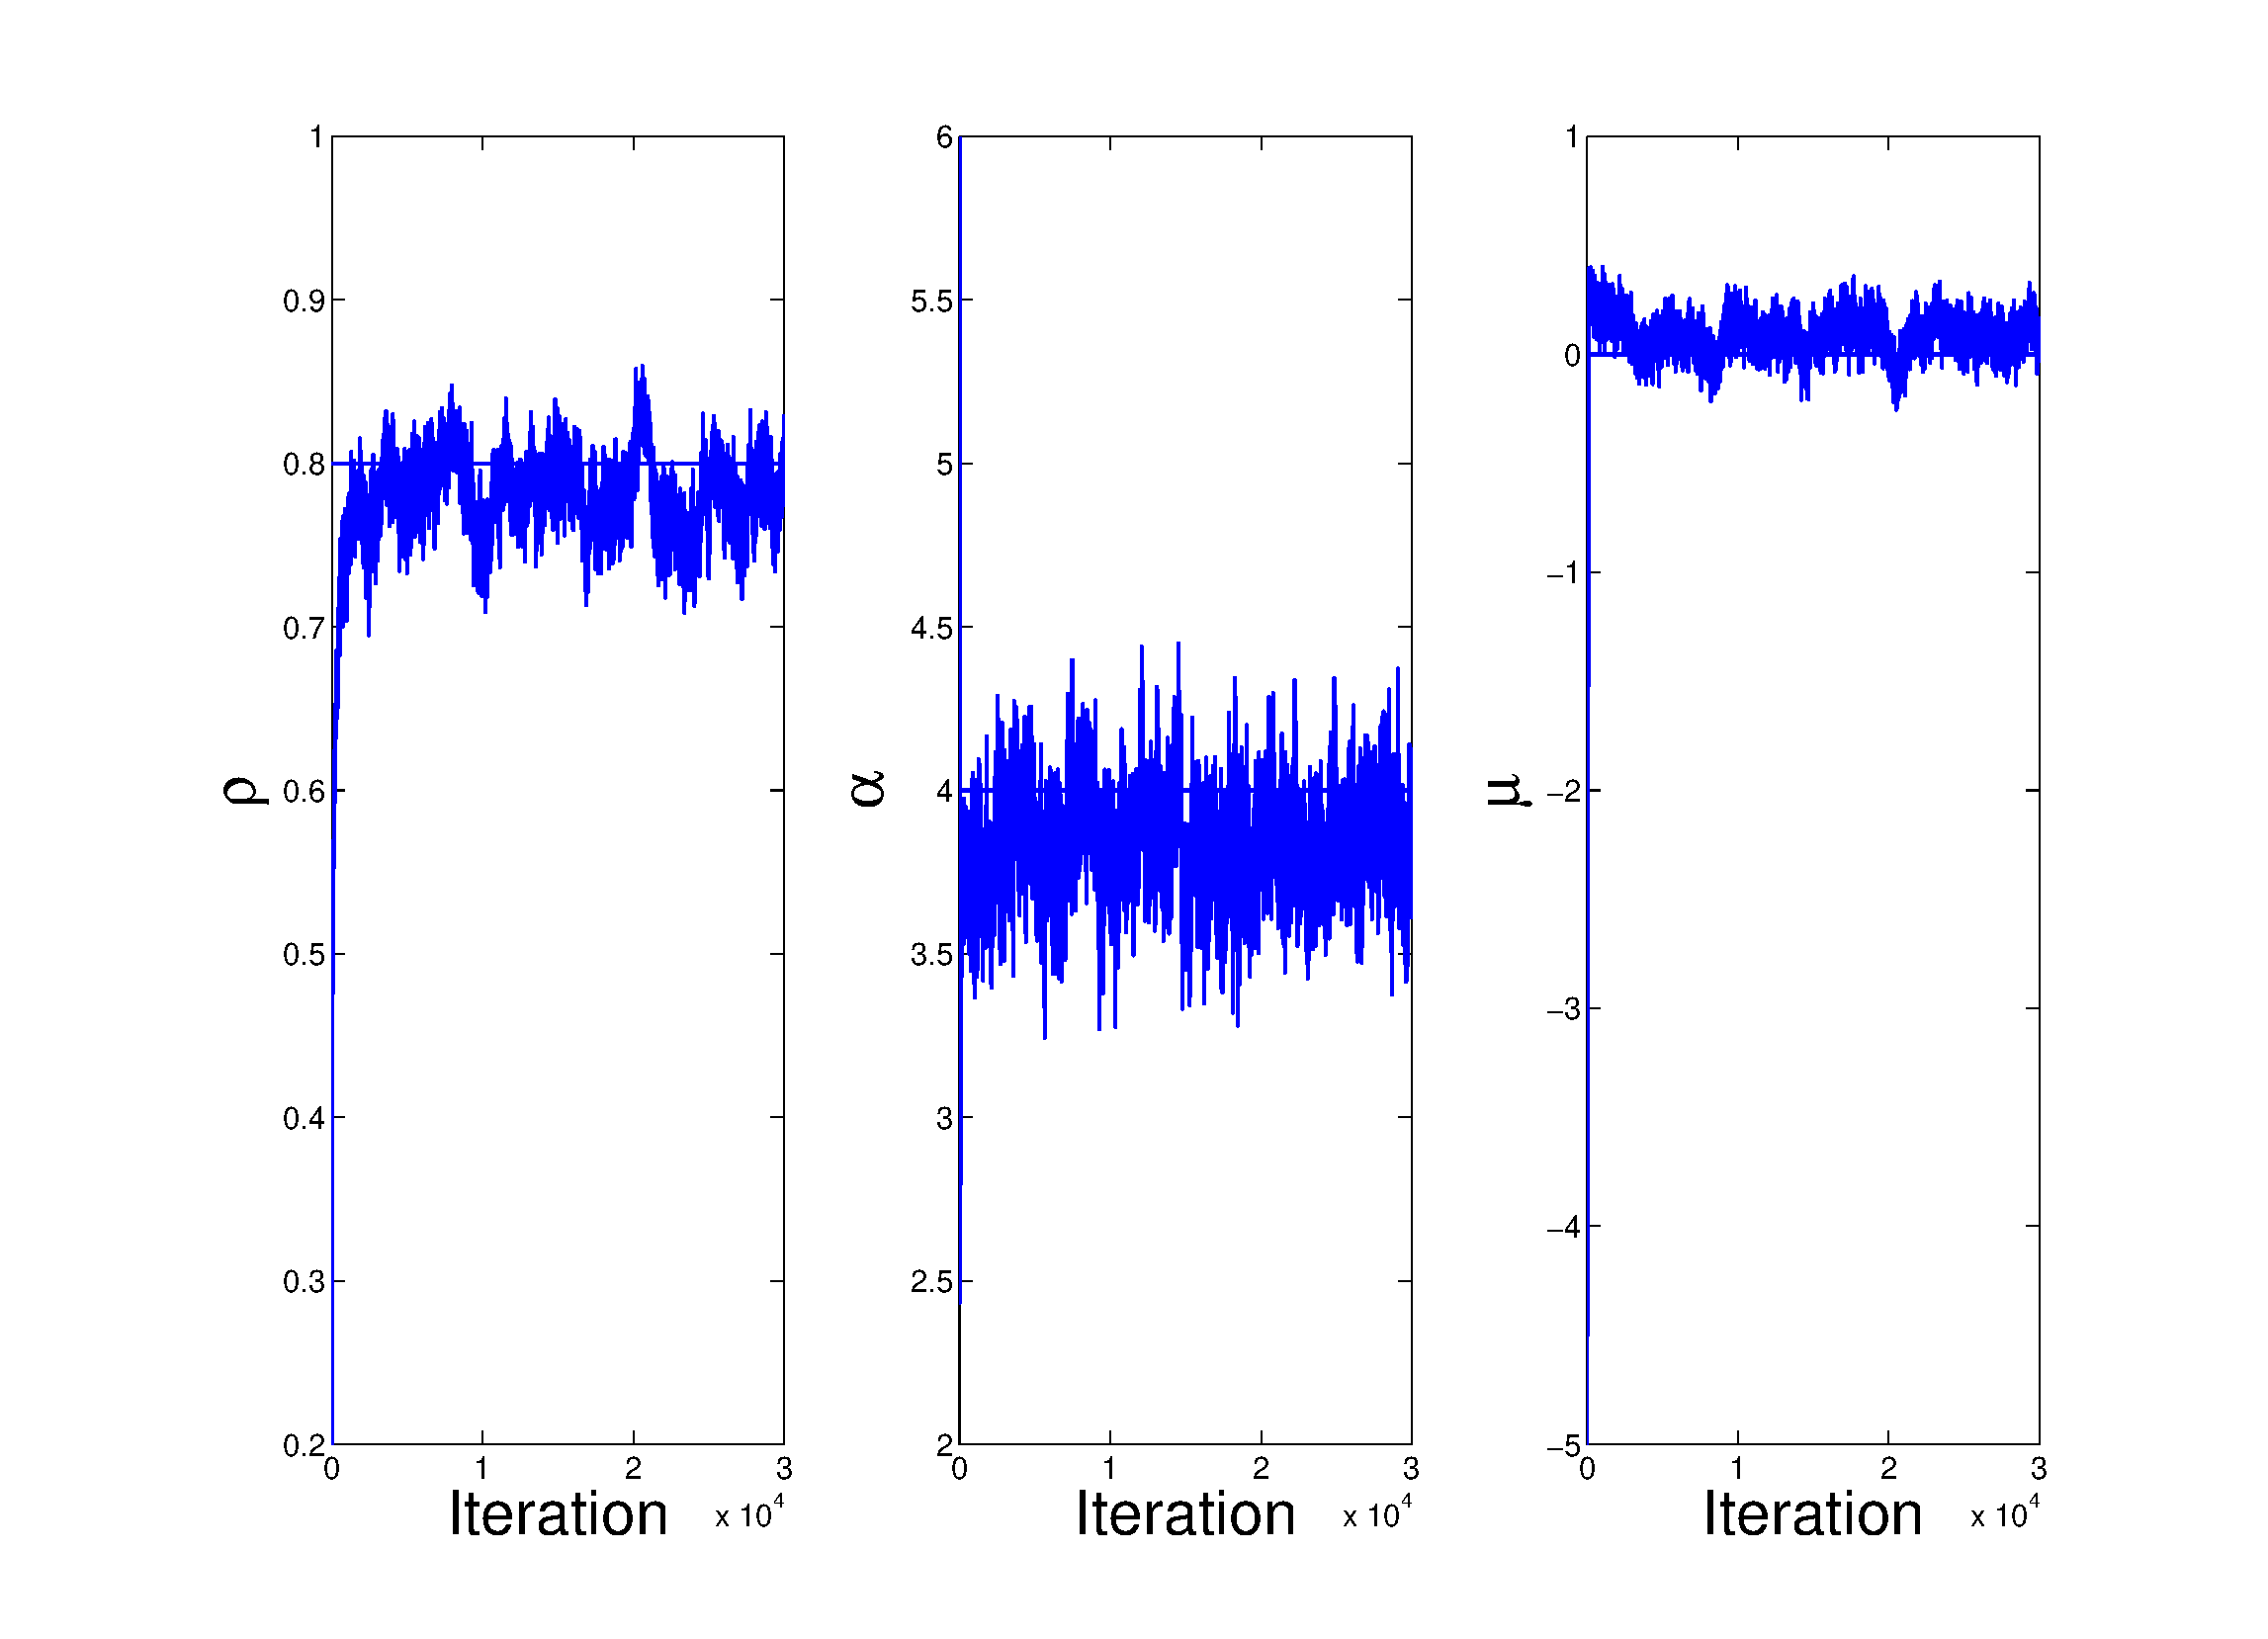
\includegraphics[height=3in,width = 5in]{./Figures/fixbeta.eps}
	\caption{The trajectory of the Gibbs sampler of each of the parameters of interest.}
	\label{Fig:Gibbsfixbeta}
\end{figure}

Figure \ref{Fig:Gibbsfixbeta} shows that the Gibbs sampler is able to converge within $5000$ iterations.
However, the states and parameters are normally highly correlated in the state space model, which often results
in poor mixing. This is because highly correlated variables often lead to small moves when sampling each of the variables. Hence the algorithm exhibits poor convergence in the joint space. More details of the convergence performance can be shown through the autocorrelation function (ACF), which measures the correlation between samples.

\begin{figure}[ht]
	\centering
	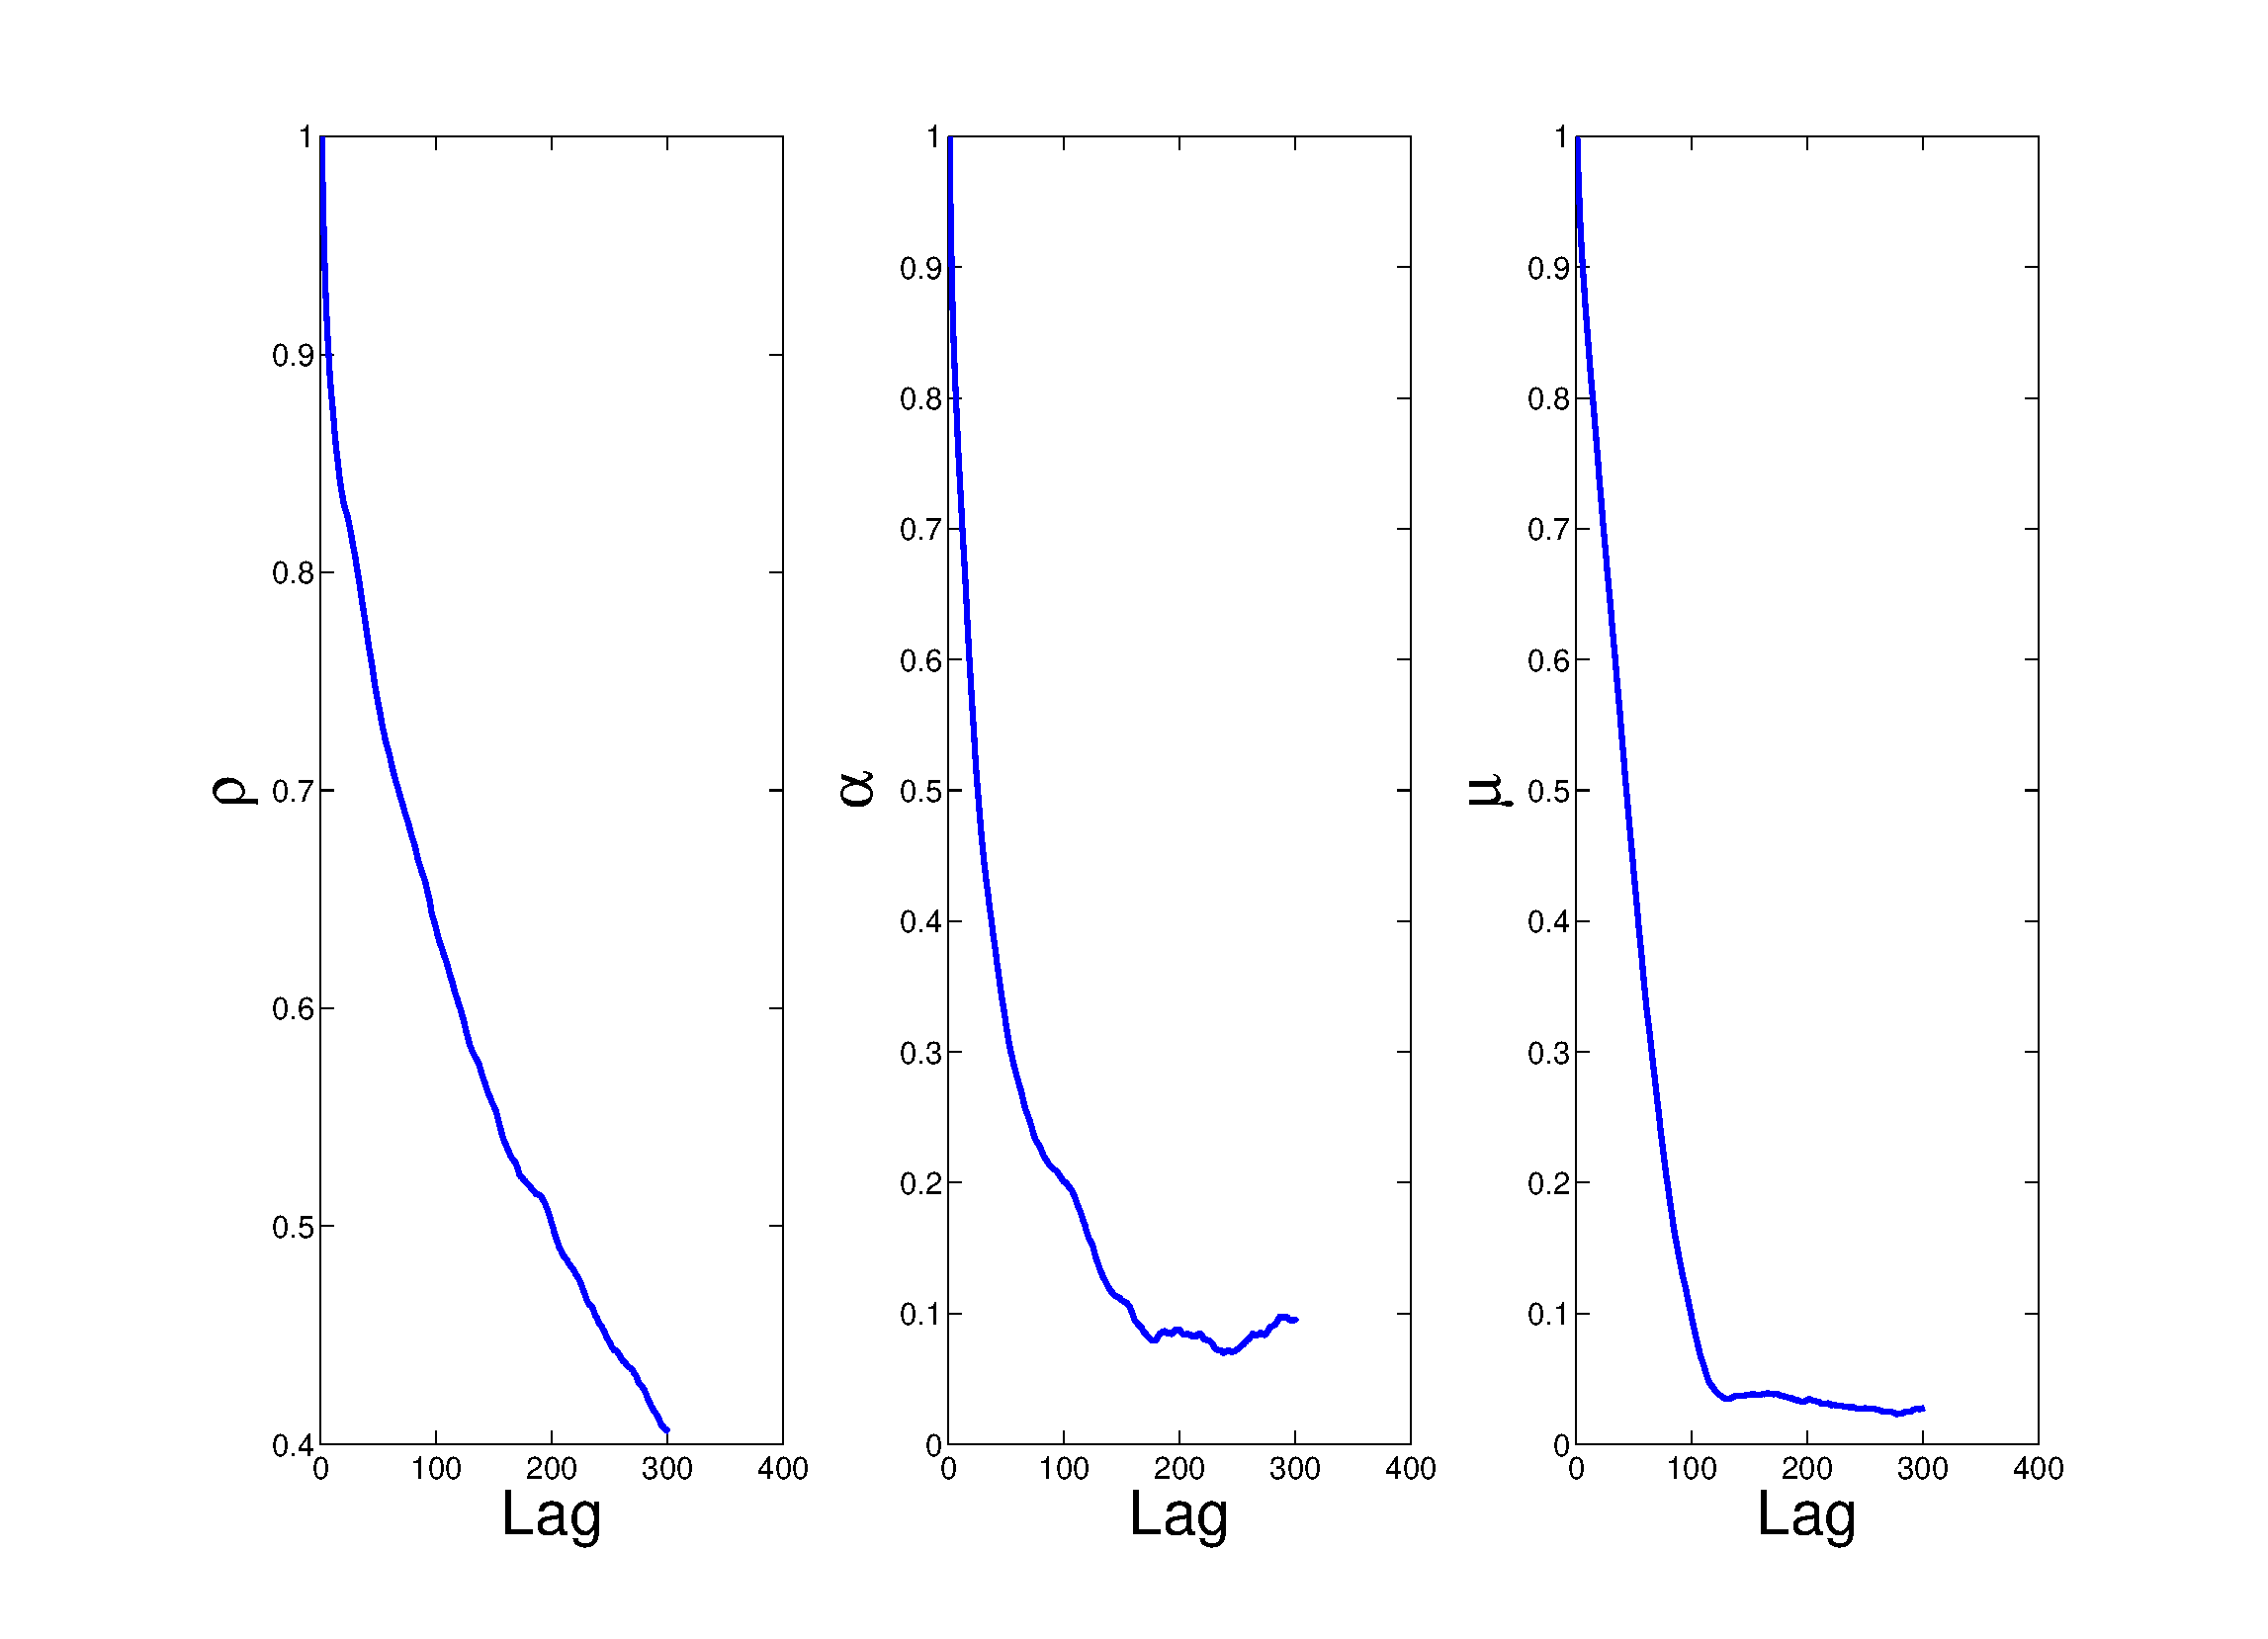
\includegraphics[height=3in,width = 5.0in]{./Figures/fixbetaacf.eps}
	\caption{The ACF of each sample path during first 300 lags.}
	\label{Fig:Gibbsacf}
\end{figure}

In this case, as shown in Figure \ref{Fig:Gibbsacf}, when compared with $\alpha$ and $\mu$, $\rho$
exhibits poor convergence. The  ACF of $\rho$ decreases slowly, because it is highly correlated with the states. In
contrast, the ACF of $\alpha$ and $\mu$ decreases fast and becomes stationary within 200 lags.
The  ACF of $\mu$ in particular drops down and keeps at a lower value when compared with $\rho$ and $\alpha$,
as $\mu$ is independent from the states and other parameters.

In our future work, in order to overcome the difficulty mentioned above, we would like to explore more
sophisticated approaches approaches for the state estimation.
For instance, using the filtering and smoothing algorithms to generate new states samples. One may also utilize a Hybrid Monte Carlo approach which has been shown to exhibit good performance in a state-space model setting \cite{Chen_2000}.

\section{Further results}

\subsection{Offline VB}
	
We supplement the results shown in the submitted work by showing those of the state and $\betab$ in addition to other 3 parameters. All the states and 23 parameters in this case were estimated very well with the true values well within the confidence bounds. Graphical results are shown in Fig.~\ref{fig:stateVB} and \ref{fig:parVB}

 \begin{figure}[h!]
 \begin{center}
 %\framebox[4.0in]{$\;$}
   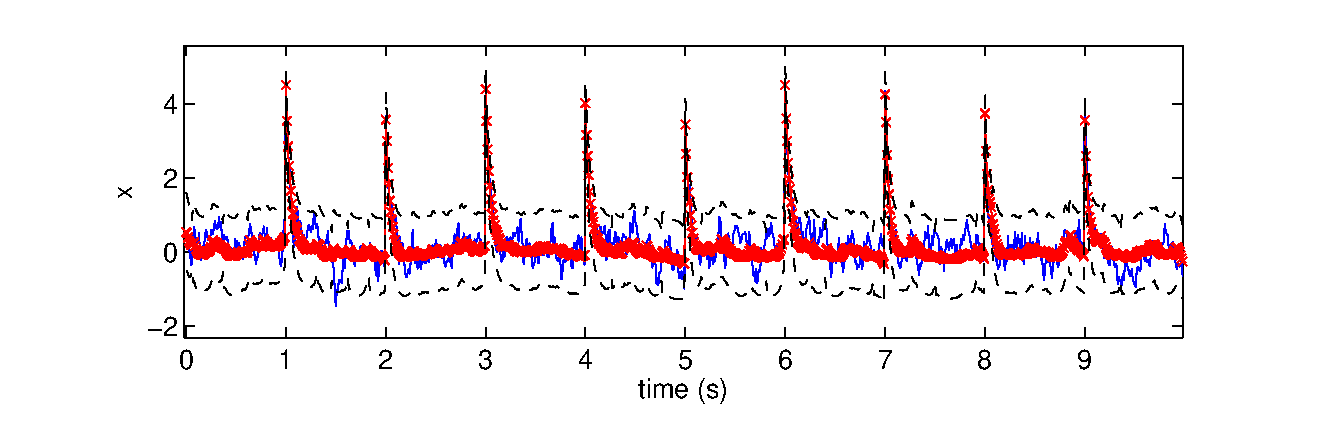
\includegraphics[width = 6in]{./Figures/stateVB.eps}

 \end{center}
 \caption{True state (solid blue line) and mean estimated state (marked red line). The true state lies consistently within the 99\% confidence intervals (dashed black line).}  \label{fig:stateVB}
 \end{figure}
 	

\begin{figure}[ht]
\begin{center}
  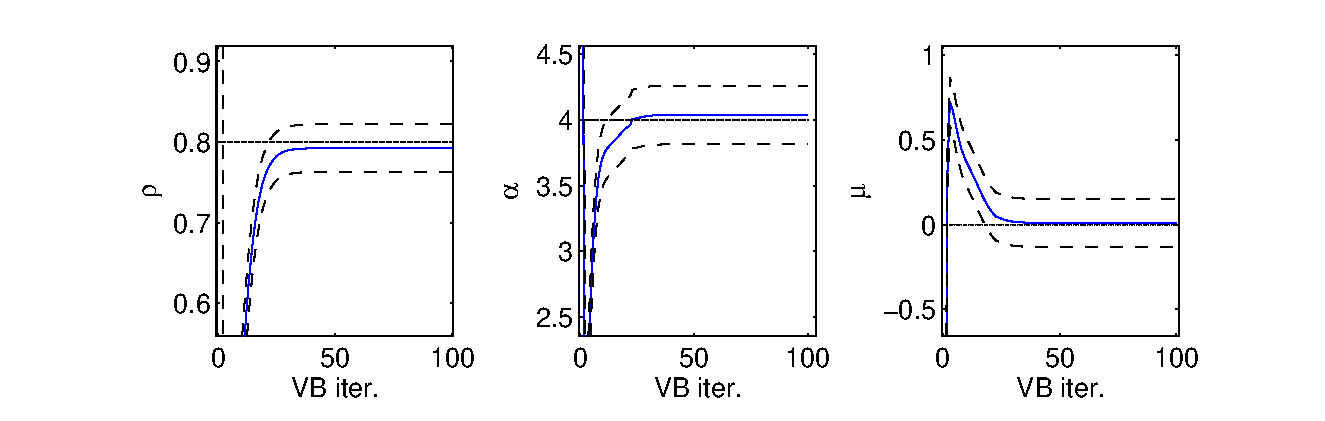
\includegraphics[width = 6in]{./Figures/parVB.eps}
   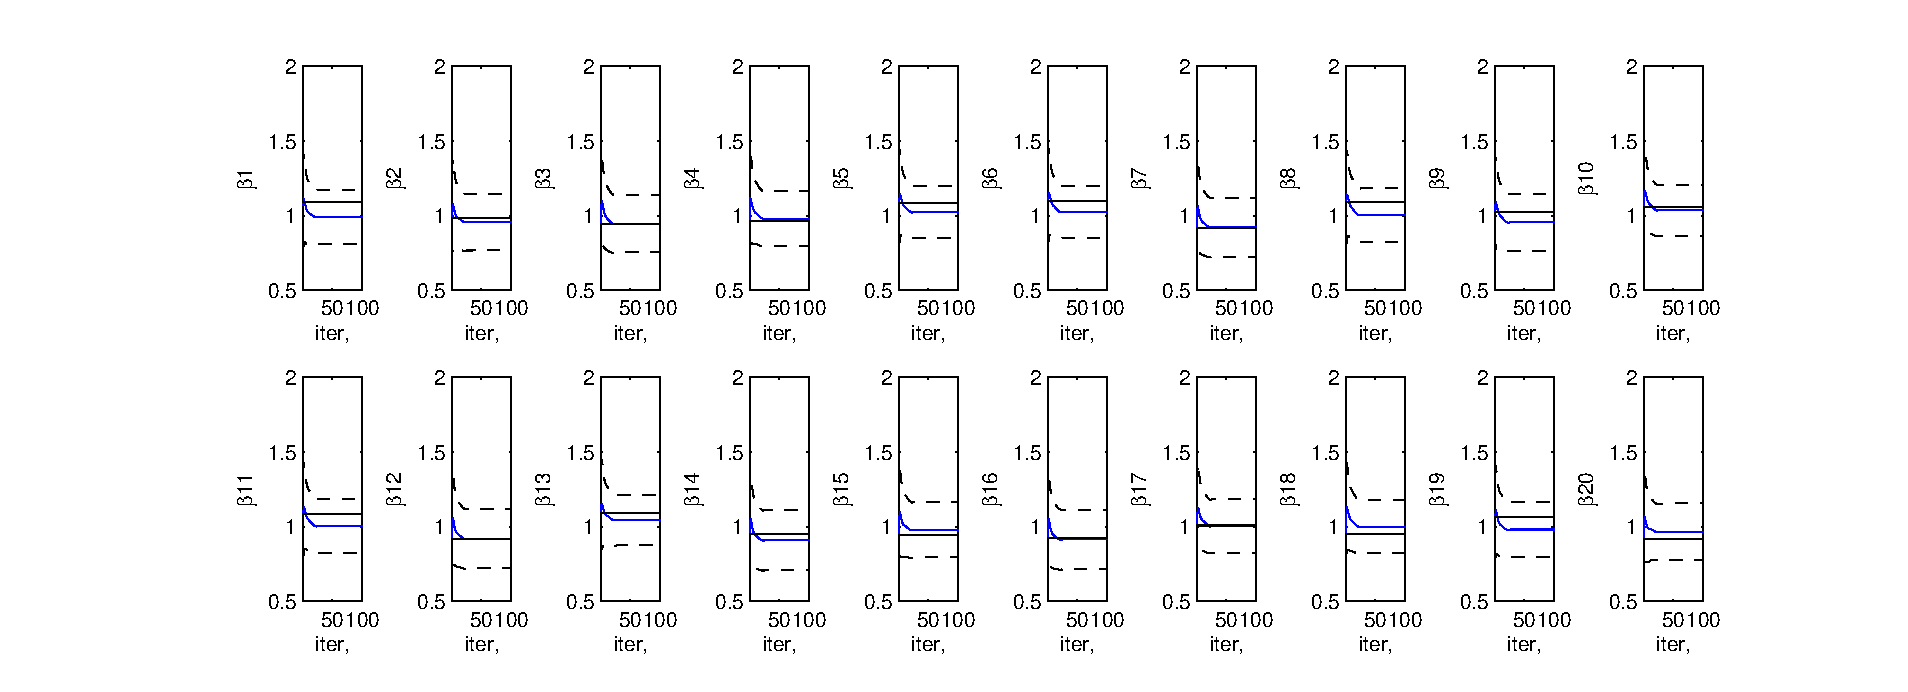
\includegraphics[width = 6in]{./Figures/betaVB.eps}
\end{center}
\caption{Mean estimates and $99\%$ confidence intervals over 100 VB-EM iterations. The parameters converge in distribution to reasonable estimates independent of initial conditions.} \label{fig:parVB}
\end{figure}

\subsection{Online parameter tracking of a parameter from point process observations}

 We initially applied the online VB filter to the same example discussed previously. The nature of the data typical in these types of models required some further intervention for correct estimation using the online filter. In the absence of hidden state, the observed events in the output are due to the background firing rate $\mu$ and there is little or no information about $\rho, \alpha$ and $\betab$ in these regions. On the other hand, the hidden state governs the output in regions when it is substantial, that is, in time intervals close to an input spike. In these areas there is significant information about $\rho, \alpha$ and $\betab$. We hence chose to update our parameter distributions only in regions where there is ample information about the relevant parameters. This was found to facilitate convergence and overall performance. The same was carried out when dealing with real data in the submitted work.

 For this study we assumed $C=80$ and that $\betab$ and $\mu$ were pre-determined from a previous offline analysis and assumed to be constants.  The choice of the forgetting factors was carried out by trial and error such that a parameter change could be tracked without compromising stability in the online estimates. We subsequently chose $\lambda^\rho = 0.8$ and $\lambda^\alpha = 0.8$. The result for the successful tracking a sudden change in the true value of $\rho$ from 0.8 to 0.6 is shown in Fig.~\ref{fig:oltrack}.

 \begin{figure}[ht]
 \begin{center}
   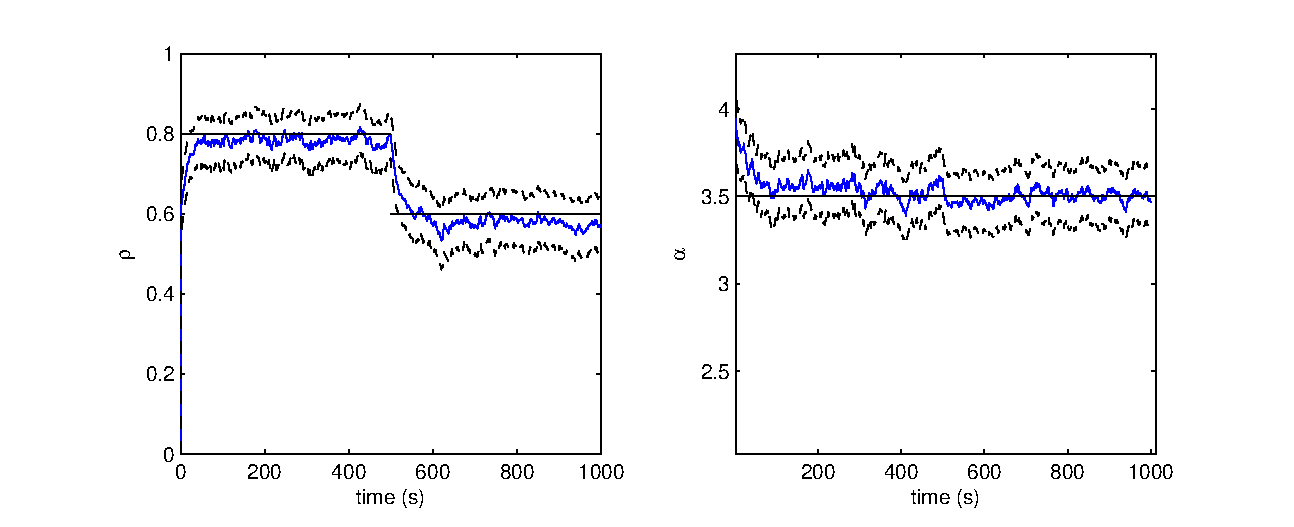
\includegraphics[width = 6in]{./Figures/onlinetrack.eps}
 \end{center}
 \caption{Online tracking of sudden change in parameter the true parameter (level black line) $\rho$ at time $t = 500s$. In this example $\mu$ and $\betab$ where assumed constant and known from previous offline analysis of the system. Note how the change in the estimate (tracking blue line) $\rho$ causes a slight change in the behaviour of the estimate of $\alpha$. This is expected from the assumed correlation between the two variables. The 99\% confidence intervals (black dashed lines) are seen to enclose the true value upon the filter reaching a steady behaviour.} \label{fig:oltrack}
 \end{figure}

\bibliography{./spikeSSM}

\vfill

\end{document} 